
\section{\label{sec:03} Analyse simplifiée de l’asservissement du drone}

La structure générale de commande du drone est constituée de différents éléments présentés de manière schématique en \autoref{fig_ccinppsi2022:15}. On y retrouve :
\begin{itemize}
\item le contrôleur de position qui génère les valeurs de consigne en attitude 
(angles de roulis $\theta_R$, 
de tangage $\theta_T$ 
et de lacet $\theta_L$)
et de poussée des moteurs ;
\item­ le contrôleur d’attitude, qui permet de contrôler l’orientation du drone dans l’espace;
\item­ l’estimateur d’attitude, qui est composé de gyroscopes et accéléromètres pour estimer
les angles de roulis $\theta_R$, tangage $\theta_T$ et d’un magnétomètre afin d’obtenir le cap du drone
(angle de lacet $\theta_L$);
­ l’estimateur de position qui est composé de la caméra embarquée et d’un baromètre
afin d’estimer les positions et vitesses du drone.
\end{itemize}

\begin{obj}
L’objectif de cette partie est de vérifier que les performances de contrôle en roulis sont
conservées lors du passage de l’ouverture et lors de l’activation du mécanisme de repliement/dépliement des bras. On se limite pour cela à la structure encadrée en pointillés de la
\autoref{fig_ccinppsi2022:15}.
\end{obj}


\begin{figure}[H]
\centering
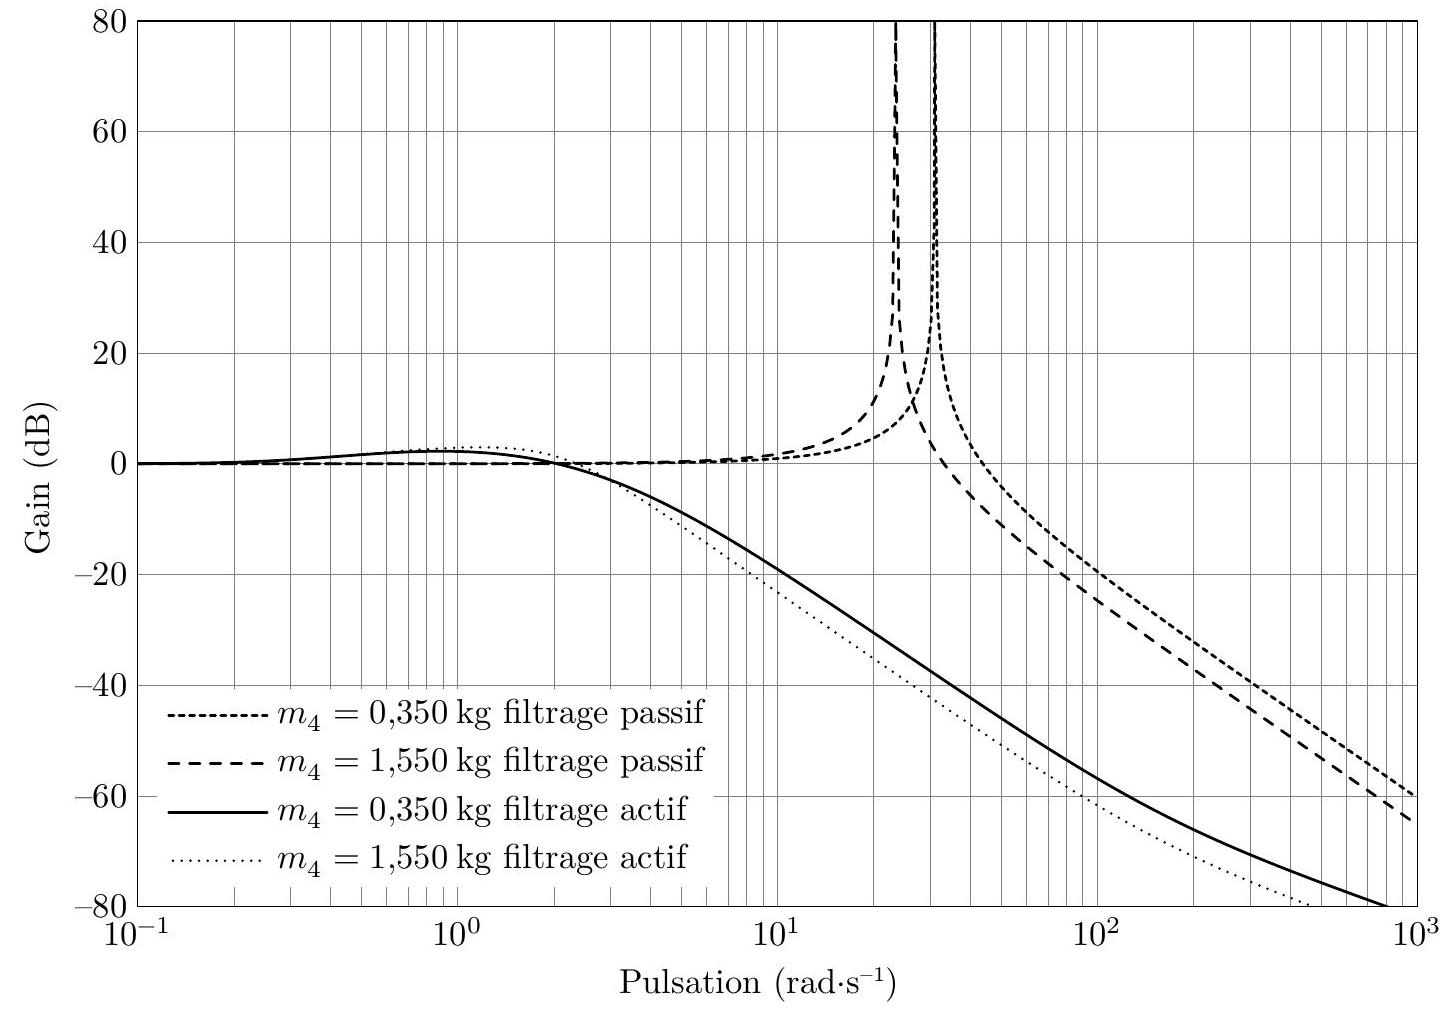
\includegraphics[width=.8\linewidth]{fig_15}
\caption{\label{fig_ccinppsi2022:15} Structure de commande du drone}
\end{figure}

\subsection{­Modélisation du comportement des moteurs brushless}

Chaque hélice du drone est actionnée par un moteur brushless, lui-même alimenté par un
ESC (Electronic Speed Controller). L’ESC est un contrôleur qui permet de faire varier la
vitesse de rotation du moteur à l’aide d’une commande PPM (Pulse Position Modulation). Il
génère ainsi les signaux pour les trois phases du moteur.

En vue d’établir un modèle de comportement des moteurs brushless, la vitesse de rotation du
moteur $\omega_M(t)$ en \si{tr/min} est mesurée pour une variation $u(t)$ de type échelon de la commande
PPM de \SI{40}{\%} puis de 80\% sans unité. Cette évolution est donnée sur la figure du DR de la
question \ref{q_ccinppsi2022:26}.

Suite à cet essai, on propose de modéliser le comportement du moteur brushless par celui
d’un système du premier ordre, reliant $\Omega_M(p)$ la transformée de Laplace de la vitesse de rotation à
$U(p)$ la transformée de Laplace de la commande PPM. On note $\indice{H}{mot}(p) = \dfrac{\Omega_M(p)}{
U(p)}$ la fonction de transfert du moteur.

%Q26
\question{\label{q_ccinppsi2022:26} Justifier le modèle de comportement retenu pour $\indice{H}{mot}(p)$ et déterminer ses caractéristiques (valeurs numériques et unités à préciser). Faire apparaître sur la figure du DR
les tracés permettant de déterminer les caractéristiques de $\indice{H}{mot}(p)$.}
\ifprof
\begin{corrige}
\end{corrige}
\else
\fi

\subsection{Modélisation du comportement des hélices}
Afin d’obtenir un modèle fiable pour le contrôle du drone, les composantes de poussée
$T$ et de traînée $Q$ de l’action de l’air sur l’hélice sont identifiées pour le couple moteur/
hélice grâce à un banc d’essai. Ce banc d’essai, \autoref{fig_ccinppsi2022:17}, est équipé de deux capteurs
d’effort $C1$ et $C2$, chacun muni de 4 jauges de déformation, et d’un capteur optique pour
mesurer la vitesse de l’hélice. On rappelle, \autoref{fig_ccinppsi2022:16}, qu’un capteur d’effort avec les jauges
de déformation ainsi positionnées et orientées sur le corps d’épreuve du capteur permet
d’accéder à la valeur de l’effort $F$ appliqué sur le capteur.


%Q27
\question{\label{q_ccinppsi2022:27} Justifier la nécessité de décaler l’axe de rotation du moteur de l’axe du capteur d’effort
$C1$ d’une distance $d_y$ et en déduire quel capteur d’effort $C1$ ou $C2$ permet de mesurer
quelle composante de l’action (effort de poussée $T$ ou moment de traînée $Q$).}
\ifprof
\begin{corrige}
\end{corrige}
\else
\fi

\begin{figure}[H]
\centering
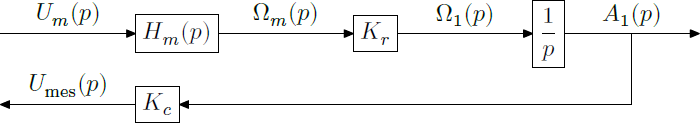
\includegraphics[width=.35\linewidth]{fig_16}
\caption{\label{fig_ccinppsi2022:16} Capteur d’effort. Deux jauges visibles au dessus, les deux autres en dessous}
\end{figure}

\begin{figure}[H]
\centering
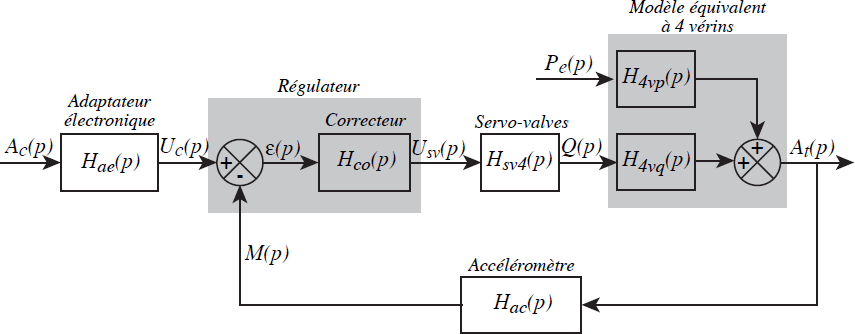
\includegraphics[width=.9\linewidth]{fig_17}
\caption{\label{fig_ccinppsi2022:17} Vue et schéma du banc d’essai pour déterminer les composantes $T$ et $Q$ de
l’action de l’air sur l’hélice en fonction de la vitesse de rotation de l’hélice}
\end{figure}

Les différentes mesures permettent de déterminer les évolutions de l’effort de poussée $T$ et
du moment de traînée $Q$ en fonction de la vitesse de rotation $\omega_1$ de l’hélice. Ces évolutions
sont présentées sur les figures du DR de la question \ref{q_ccinppsi2022:28}. Les mesures confirment une évolution
quadratique de $T$ et $Q$ en fonction de $\omega_1$, avec :
$T = c_T \omega_1^2$ avec $c_T = \SI{1e-6}{N/(rad/s)^2}$ et
$Q = c_Q \omega_1^2$ avec $c_Q = \SI{9.8e-6}{N/(rad/s)^2}$ 
où $c_T$ et $c_Q$, les coefficients de poussée, respectivement de traînée, sont obtenus par régression linéaire.

Afin de pouvoir modéliser le comportement de l’asservissement en roulis du drone lors du
passage de l’ouverture, il est nécessaire de proposer un modèle de comportement linéarisé
de chacun des composants du drone et notamment des hélices. On se place pour cela autour
du point de fonctionnement correspondant à la vitesse d’approche du drone de l’ouverture,
ce qui correspond à une vitesse de rotation des hélices de l’ordre de \SI{1400}{rad.s^{-1}}. On estime
que les variations de vitesse de rotation des hélices sont au maximum de $\pm \SI{500}{rad.s^{-1}}$ lors
des corrections d’attitude et de cap nécessaires au passage de l’ouverture.

%Q28
\question{\label{q_ccinppsi2022:28} Proposer un modèle de comportement linéarisé de la variation de l’effort de poussée
$\Delta T$ et $\Delta Q$ en fonction de la variation de vitesse de rotation $\Delta \omega_1$ autour du point de
fonctionnement étudié ($\omega_1 \simeq \SI{1400}{rad.s^{-1}}$) et valable dans le domaine de variation de
$\pm \SI{500}{rad.s^{-1}}$ considéré. Laisser apparents sur les courbes du DR les tracés permettant de justifier votre démarche.}
\ifprof
\begin{corrige}
\end{corrige}
\else
\fi

\subsection{Analyse du contrôleur d’attitude en roulis}

Dans cette sous­partie, on s’intéresse au réglage du contrôleur d’attitude en roulis dans le
cas d’une commande en échelon sans perturbation. Puis, nous verrons comment se comporte le drone en roulis lors du passage de l’ouverture (ajout d’une perturbation) et enfin
son comportement lors du repliement des bras. L’objectif est de s’assurer que le réglage du
contrôleur d’attitude permet de conserver, dans une certaine mesure, le contrôle en roulis
lors du passage de l’ouverture et lors du repliement/dépliement des bras.

\begin{figure}[H]
\centering
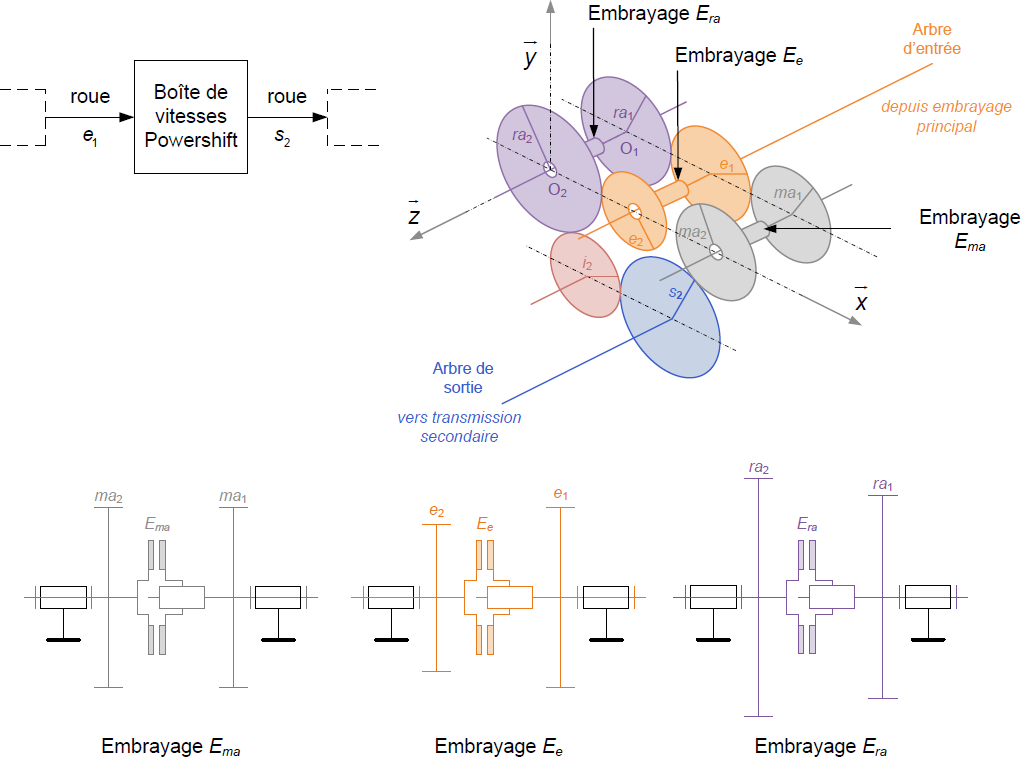
\includegraphics[width=.8\linewidth]{fig_18}
\caption{\label{fig_ccinppsi2022:18} ­ Représentation simplifiée par schéma-blocs de l’asservissement du drone en
roulis, angle $\theta_R$ en degrés}
\end{figure}

L’asservissement du drone en roulis, angle $\theta_R$, est représenté par le schéma bloc de la
\autoref{fig_ccinppsi2022:18}. Les performances de cet asservissement sont décrites par l’exigence Id 2 du
diagramme des exigences donné en \autoref{fig_ccinppsi2022:21} annexe 1. Les grandeurs indiquées sur le
schéma bloc de la \autoref{fig_ccinppsi2022:18} représentent les transformées de Laplace des grandeurs obtenues pour des variations autour du point de fonctionnement $\theta_R = 0\degres$. La vitesse de rotation du
drone en roulis en \si{deg/s} est notée $\Omega_R(p)$. Le contrôleur d’attitude est un correcteur de fonction de transfert $C(p)$ de sortie $U(p)$ en incréments (inc). Le comportement de l’estimateur
d’angle en roulis (composé d’un gyromètre, d’un accéléromètre et d’un système de traitement des signaux) est modélisé par un gain pur $K_E$, tel que $K_E = \SI{150}{inc/deg}$.
Le bloc adaptateur, de gain pur $K_A = K_E$, permet d’adapter la consigne de variation d’angle
de roulis $\theta_R^C(p)$ en degrés en une grandeur comparable à la mesure de l’estimateur d’angle
de roulis.
La fonction de transfert $H_S (p) = \dfrac{\Omega_R(p)}{U(p)}$ représente le comportement linéarisé autour d’un
point de fonctionnement (vol d’approche à vitesse constante) du drone dans la position bras
déplié $\gamma_1 = 90\degres$. Ce comportement a été défini, entre autres, à partir des résultats des analyses des parties précédentes.


Une simulation a permis de tracer les diagrammes de Bode de la réponse fréquentielle de
$H_S (p)$. Cette réponse est donnée sur la figure du DR de la question \ref{q_ccinppsi2022:29}, où l’on retrouve l’évolution du
gain $G_{HS}(\omega) = 20 \log |H_S (j\omega)|$ et de la phase $\Phi_{HS} (\omega) = \arg\left(H_S (j\omega)\right)$ en fonction de la pulsation $\omega$.

Compte tenu de la réponse fréquentielle de $H_S (p)$, on propose le modèle suivant pour $H_S (p)$ :
$H_S(p)=\dfrac{K_S}{1+\dfrac{2z_S}{\omega_{0S}}p+\dfrac{1}{\omega_{0S}^2}p^2}$.


%Q29
\question{\label{q_ccinppsi2022:29} Justifier le choix retenu pour l’expression de $H_S (p)$ et déterminer graphiquement les
valeurs numériques et unités des paramètres caractéristiques $K_S$ , $z_S$ et $\omega_{0S}$ . Faire apparaître sur la figure du DR, les constructions permettant de justifier les valeurs proposées.}
\ifprof
\begin{corrige}
\end{corrige}
\else
\fi


%Q30
\question{\label{q_ccinppsi2022:30} Tracer, sur la figure du DR, les courbes de gain $\indice{G}{BO}(\omega)$ et de phase $\indice{\Phi}{BO}(\omega)$ de la réponse fréquentielle de la fonction de transfert en boucle ouverte $\indice{H}{BO}(p) = \dfrac{\theta_{R}^{\text{mes}}(p)}{\varepsilon(p)}$
non corrigée, c’est-à-dire pour $C(p) = 1$. Justifier vos tracés.}
\ifprof
\begin{corrige}
\end{corrige}
\else
\fi

%Q31
\question{\label{q_ccinppsi2022:31}  Représenter, sur le DR, les marges de gain $MG$ et marge de phase $M\Phi$ de la FTBO si
elles sont définies. Conclure sur les performances de l’asservissement en roulis sans
correction (exigence Id 2).}
\ifprof
\begin{corrige}
\end{corrige}
\else
\fi

On s’intéresse tout d’abord à l’effet de l’action proportionnelle du contrôleur d’attitude et on
pose $C(p) = K_P$.


%Q32
\question{\label{q_ccinppsi2022:32} Déterminer graphiquement la valeur à donner à $K_P$ pour vérifier le critère de stabilité.}
\ifprof
\begin{corrige}
\end{corrige}
\else
\fi


D’après les résultats des simulations, l’action proportionnelle du contrôleur d’attitude permettrait le respect des performances en roulis dans le cas de vol non perturbé. La prise en
compte des perturbations est complexe à modéliser sur un tel système, aussi on considère
en première approximation que les perturbations en vol contribuent à une variation de vitesse
de roulis $P(p)$, modélisée par la suite comme une perturbation de type échelon d’amplitude $P_0$
(\autoref{fig_ccinppsi2022:19}).

\begin{figure}[H]
\centering
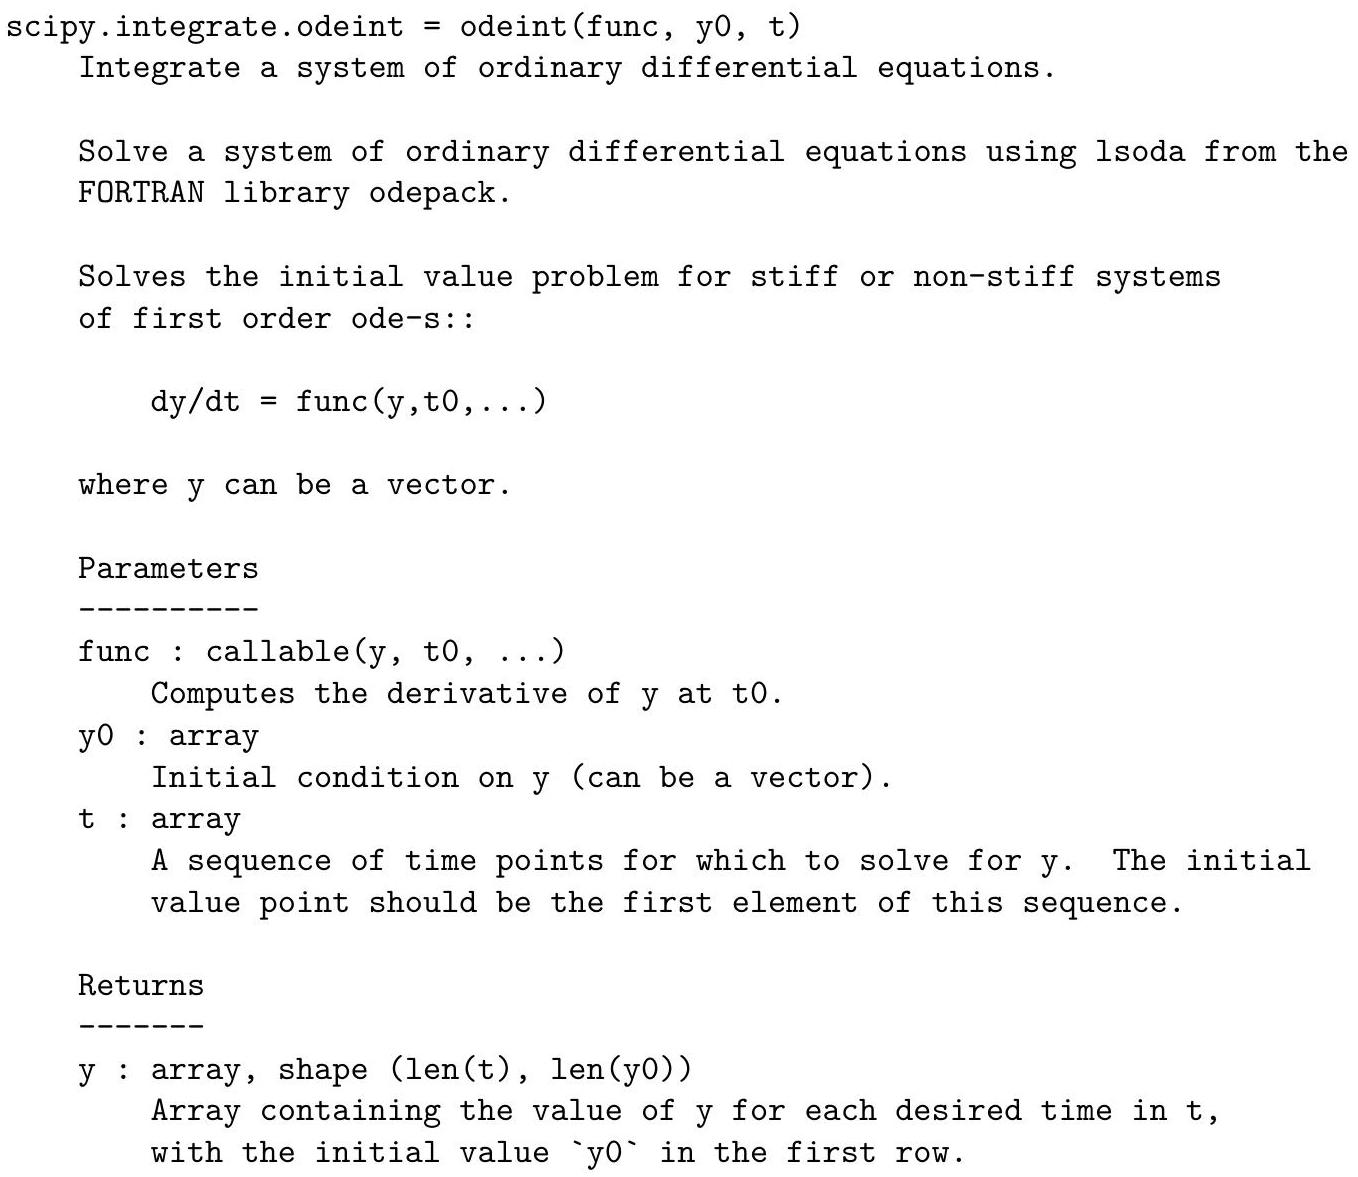
\includegraphics[width=.8\linewidth]{fig_19}
\caption{\label{fig_ccinppsi2022:19} Représentation par schéma bloc avec prise en compte des perturbations en vol}
\end{figure}


%Q33
\question{\label{q_ccinppsi2022:33} Déterminer l’expression de $\theta_R(p)$ en fonction de $\theta_R^C(p)$
 et de $P(p)$. On rappelle que $C(p) = K_P$ et $H_S (p)$ est définie par l’équation (2).}
\ifprof
\begin{corrige}
\end{corrige}
\else
\fi

%Q34
\question{\label{q_ccinppsi2022:34} Déterminer l’expression de la contribution de la perturbation de type échelon d’amplitude $P_0$ sur la valeur de $\theta_R(t)$ en régime établi dans le cas où la consigne est nulle $\theta_R^C(t)=0\degres$.}
\ifprof
\begin{corrige}
\end{corrige}
\else
\fi

%Q35
\question{\label{q_ccinppsi2022:35} Quelle valeur donner à $K_P$ pour respecter le critère de précision vis-­à-­vis de la perturbation ? Conclure sur les limites de la correction proportionnelle.}
\ifprof
\begin{corrige}
\end{corrige}
\else
\fi

Il est alors décidé de mettre en place une correction proportionnelle intégrale (correcteur PI)
avec $C(p) = K_P\left(\dfrac{1+T_i p}{T_i p}\right)$. On fixe pour la suite $K_P = 0,1$.

%Q36
\question{\label{q_ccinppsi2022:36} Justifier que cette correction permet de satisfaire les critères de précision sur la
consigne et sur la perturbation.}
\ifprof
\begin{corrige}
\end{corrige}
\else
\fi

Les figures du DR de la question \ref{q_ccinppsi2022:37} donnent les résultats de la simulation du système avec la
correction proportionnelle intégrale retenue. La première donne l’évolution de $\theta_R(t)$ pour une
consigne de roulis $\theta_R^C(t)$ de type échelon d’amplitude $\theta_{R0}^C = 10\degres$ et pour une perturbation $P(t)$ de
type échelon d’amplitude $P_0 =\SI{10}{deg/s}$ appliquée en $t = \SI{2}{s}$. La seconde donne les courbes
de gain et de phase du diagramme de Bode de la réponse fréquentielle de la FTBO corrigée.

%Q37
\question{\label{q_ccinppsi2022:37} Vérifier les performances temporelles et déterminer les marges de gain et de phase
de la FTBO avec correction. Faire apparaître les constructions sur les figures du DR.
Conclure sur le réglage et le choix d’un correcteur PI.}
\ifprof
\begin{corrige}
\end{corrige}
\else
\fi

Des essais en vol ont été réalisés avec le réglage précédent pour la partie roulis du contrôleur
d’attitude. Ces essais décrivent le comportement en roulis du drone lors du repliement des
bras, du passage de l’ouverture et du dépliement des bras. Les évolutions de l’angle de
roulis (en degrés) et de la vitesse de rotation en roulis (en \si{deg/s}) du drone sont données
en figure 20 pour 10 essais. Sur cette figure, l’origine des temps, $t = \SI{0}{s}$, correspond au
déclenchement de la procédure de repliement des bras, l’ouverture est traversée par le drone
à partir de l’instant $t = \SI{0,25}{s}$ jusqu’à $t = \SI{0,5}{s}$ et le dépliement des bras débute pour $t = \SI{0,5}{s}$.

\begin{figure}[H]
\centering
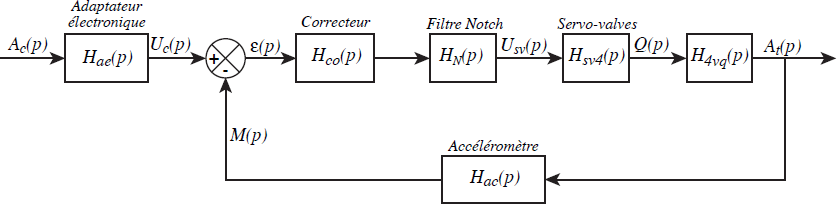
\includegraphics[width=.8\linewidth]{fig_20}
\caption{\label{fig_ccinppsi2022:20} ­Évolutions de l’angle de roulis (en degrés) et de la vitesse de rotation en roulis
(en \si{deg/s}) du drone sont donnée pour 10 essais.}
\end{figure}

%Q38
\question{\label{q_ccinppsi2022:38} Conclure sur l’influence de la phase de repliement des bras et du passage de l’ouverture sur le comportement en roulis du drone avec la correction retenue.}
\ifprof
\begin{corrige}
\end{corrige}
\else
\fi


\newpage

\section*{Annexe 1}


\begin{figure}[H]
\centering
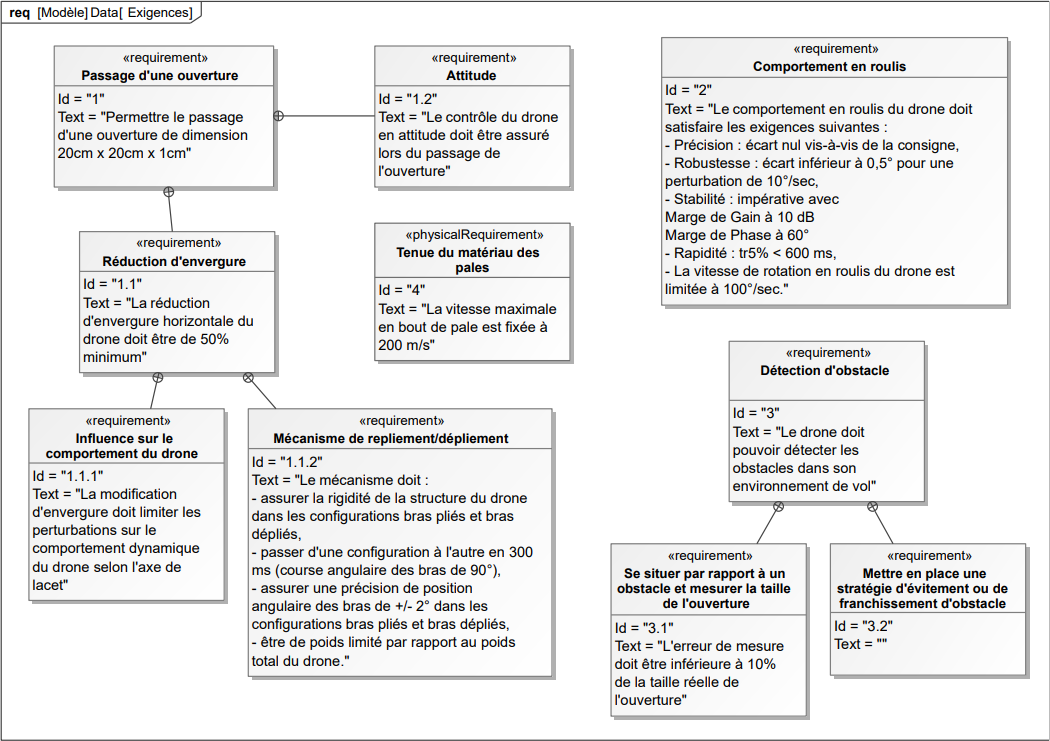
\includegraphics[width=\linewidth]{fig_21}
\caption{\label{fig_ccinppsi2022:21} Diagramme partiel des exigences liées au passage de l’ouverture de la plateforme QuadMorphing}
\end{figure}

\begin{figure}[H]
\centering
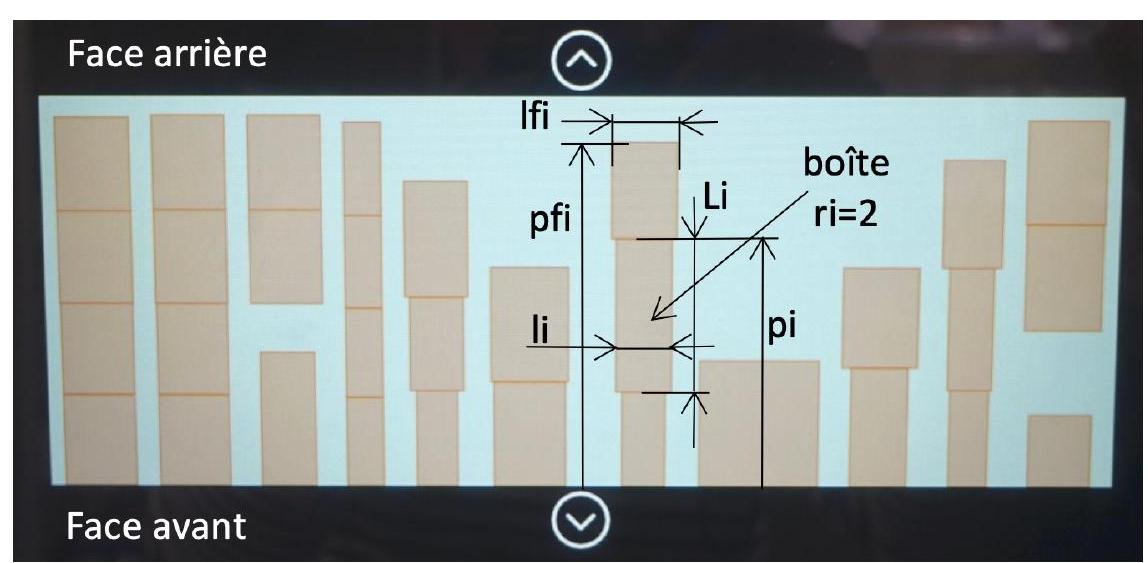
\includegraphics[width=\linewidth]{fig_22}
\caption{\label{fig_ccinppsi2022:22} Diagramme de définition des blocs de la plateforme QuadMorphing}
\end{figure}
